%\begin{figure*}[t]
%\centering
%\vspace{-2mm}
% 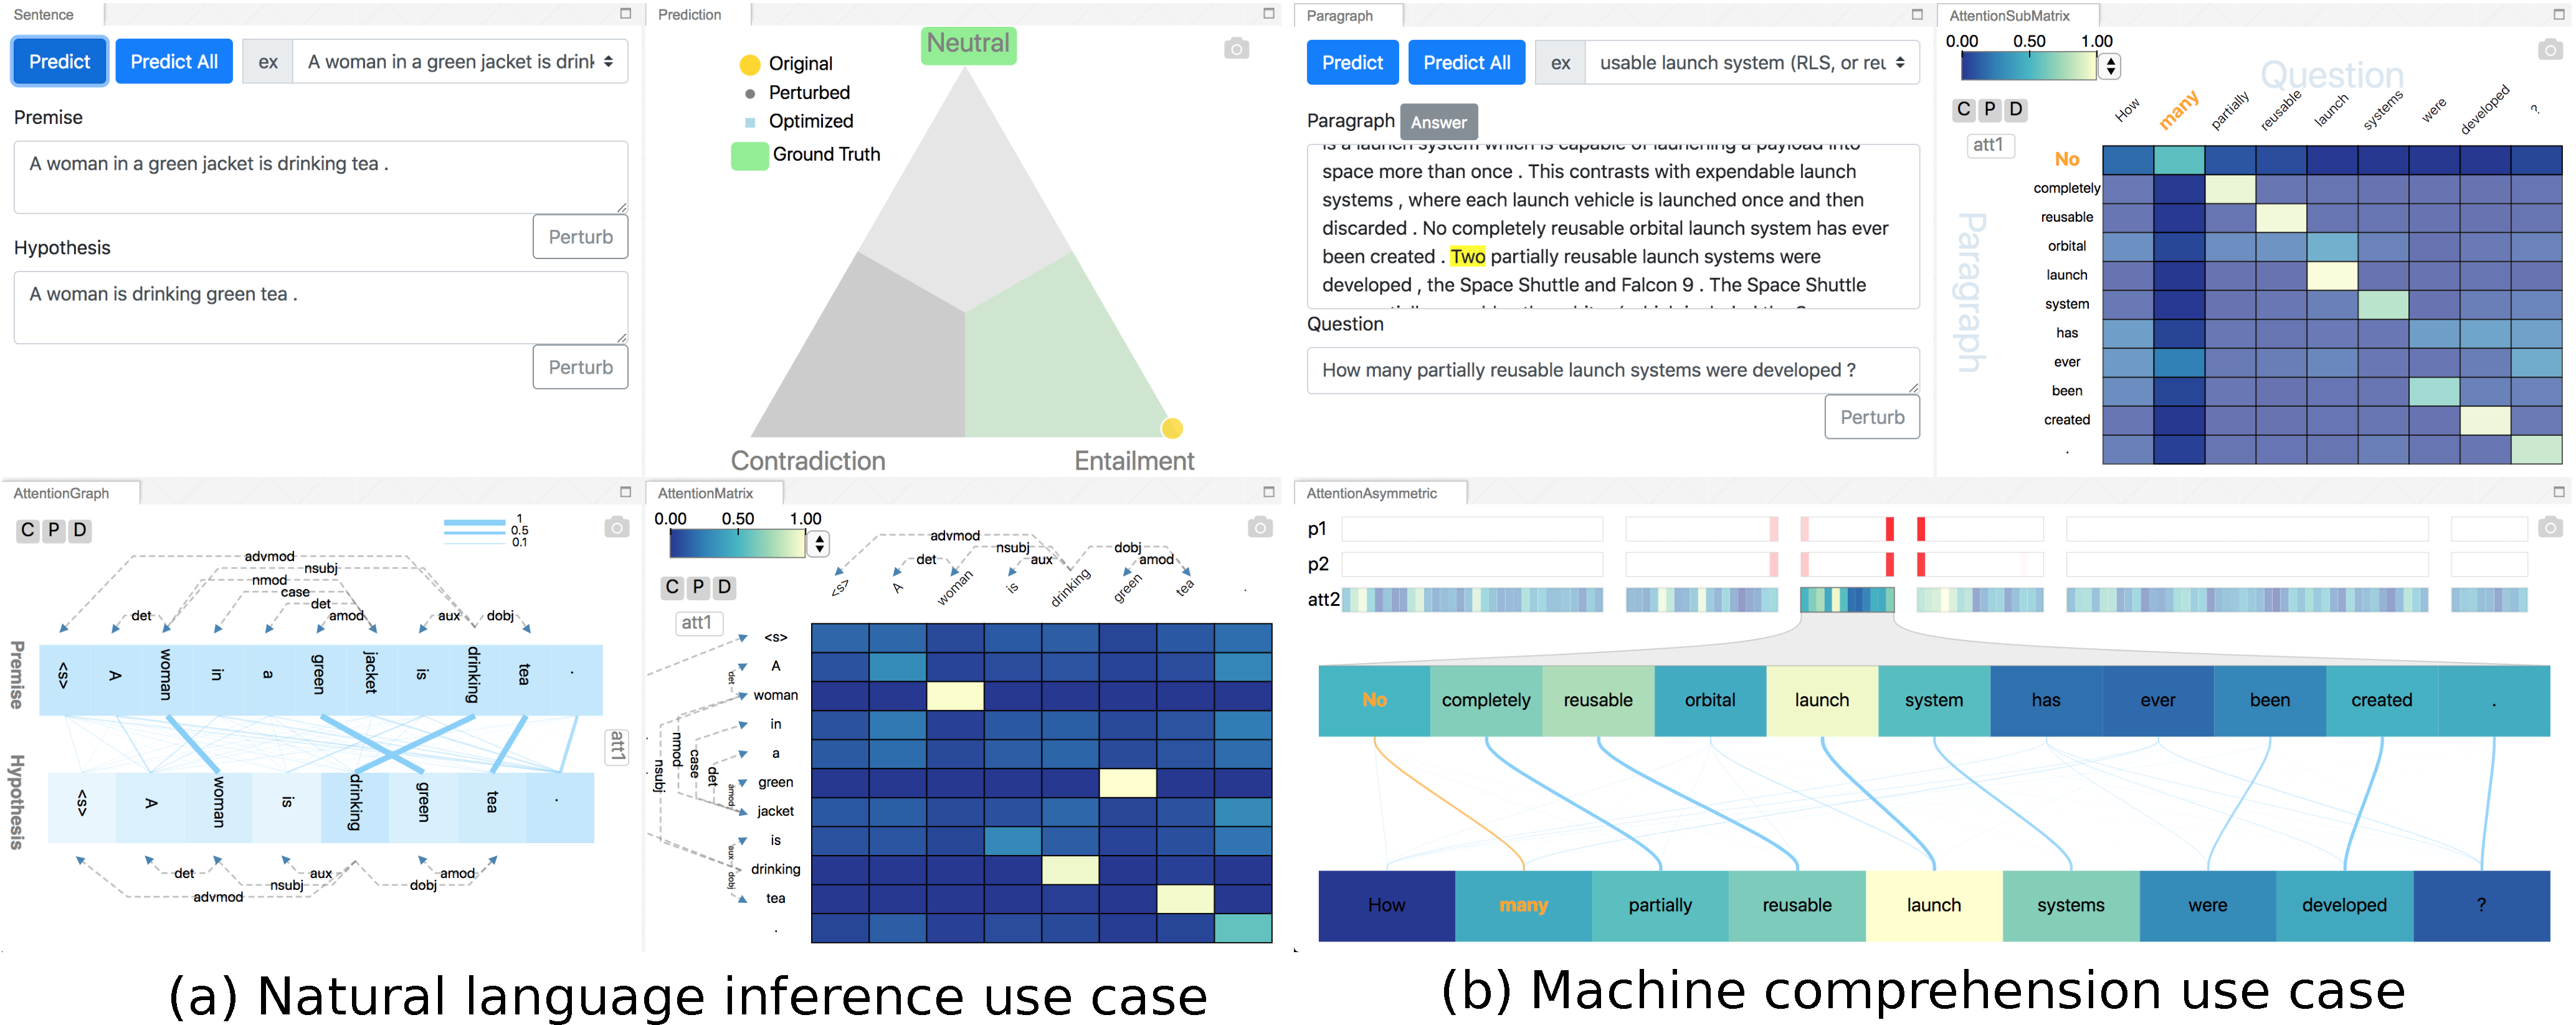
\includegraphics[width=1.0\linewidth]{NLI_MC_interface}
%  \vspace{-6mm}
% \caption{
%Illustration of different configurations for the natural language inference and machine comprehension tasks.
%}
%\label{fig:pipelineUpdate}
%\end{figure*}
\begin{figure*}[t]
\centering
 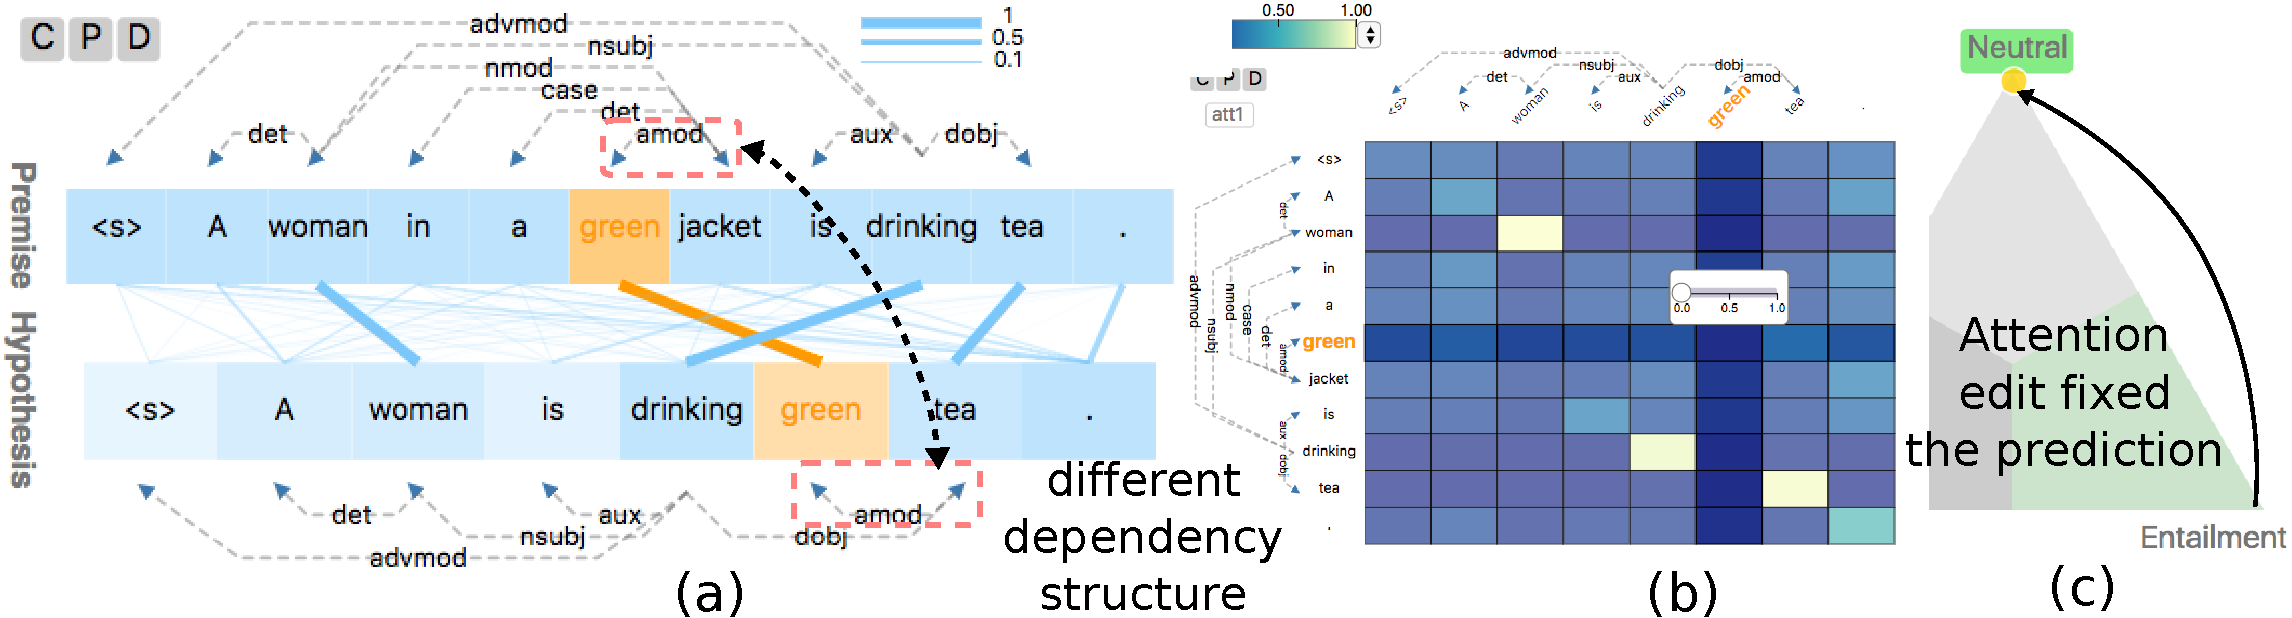
\includegraphics[width=1.0\linewidth]{NLIexample}
  \vspace{-6mm}
 \caption{
An illustration of the attention editing process.
The dependency structure is shown in (a), where the two ``greens'' decorate different nouns.
By removing the ``wrong'' alignment in (b), the original prediction \emph{entailment} is corrected to \emph{neutral} in (c).
}
\label{fig:NLIexample}
\end{figure*}

\section{Applications}
We demonstrate the proposed visualization system on the decomposable attention network~\cite{parikh2016emnlp}
for the NLI task and the BIDAF model~\cite{Seo2016} for the MC task.

\subsection{Natural Language Inference}
\label{sec:NLIexample}
The NLI task predicts the entailment relationship between a premise sentence (P) and a hypothesis sentence (H).
The attention matrix captures the alignment of words between these two sentences.
Here we give an example of how a wrong prediction can be corrected by editing attention values.  

%The model produces two attention matrices, representing alignment from premise to hypothesis, and from hypothesis to premise.
%as either \emph{entailment}, \emph{contradiction}, or \emph{neutral}.
%The model can be formalized as the following:
%%\begin{align}
%	$P^\prime, H^\prime = f(P), f(H)$,
%	$\overleftarrow{A} = P^\prime \cdot H^\prime$,
%	$\overrightarrow{A} = H^\prime \cdot P^\prime$,
%	$y = g(P, H, P^\prime, H^\prime, \overleftarrow{A}, \overrightarrow{A})$,
%%\end{align}
%where $P$ and $H$ are input embedding matrices for the premise and the hypothesis, $\overleftarrow{A}$
%and $\overrightarrow{A}$ are attentions, and $y$ is the predicted probabilities for candidate classes.
%Our system visualized the bidirectional attentions and their interaction with output distribution over labels.

As illustrated in Fig.~\ref{fig:NLIexample}(a), the input sentence pair (P:``A woman in a green jacket is drinking tea.'' H:``A woman is drinking green tea.'') is predicted to be \emph{entailment}, which is incorrect.
By examining the attention, we can see the word \emph{green} in ``\emph{green} jacket" is aligned to the \emph{green} in ``\emph{green} tea". However, these two \emph{greens} modify different nouns, which potentially leads to the wrong prediction. The grammatical structure is visually shown in the form of the dependency tree.
%i.e., \emph{green} in \textbf{P} is attached to ``jacket''.
However, the model does not have access to the syntactic information and mistakenly assumes the two \emph{greens} modify the same thing.
% (thus predict \emph{entailment}). 
%
To correct the mistake, we can edit the attention value and remove the align between these two "greens" (see (c)(b)).
As expected, the prediction label is corrected (\emph{neutral}).

\begin{figure*}[t]
\centering
 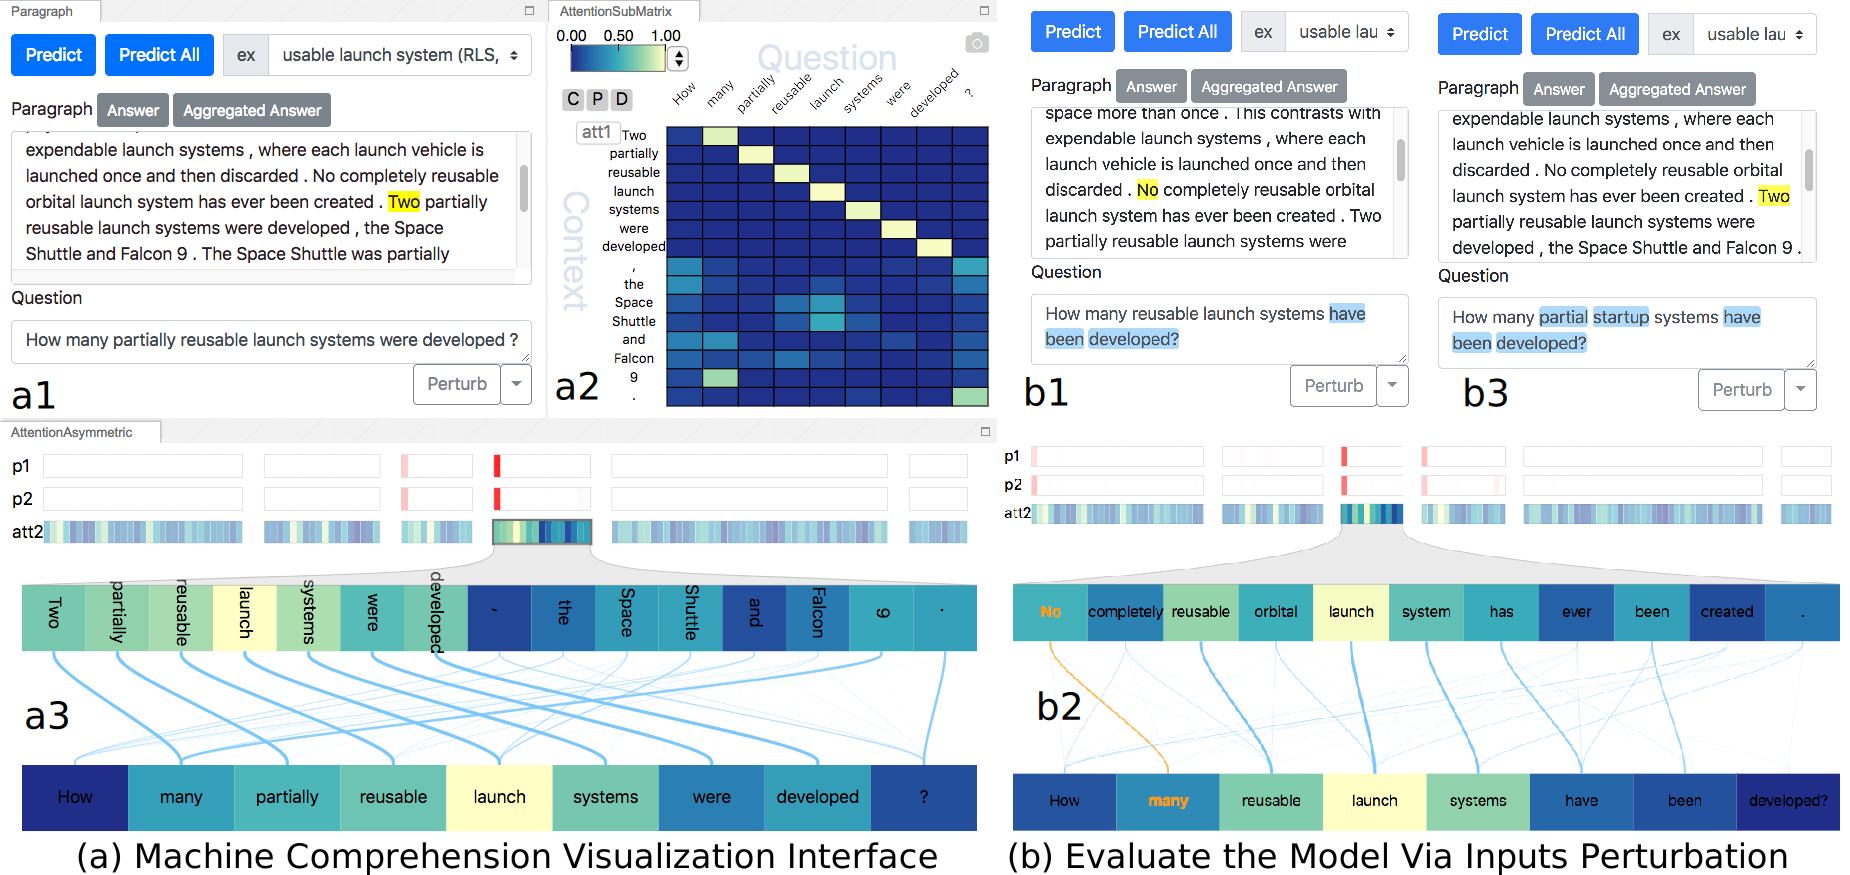
\includegraphics[width=1.0\linewidth]{MC_interface}
  \vspace{-6mm}
 \caption{
In the machine comprehension visualization interface (a), the $p1$, $p2$ colored bar (in $a3$) illustrates the predicted start and end index of the answer in the context (the deeper the red, the higher the probability). The most likely answer is shown in ($a1$). The global attention and local attention are visualized by ($a2$, $a3$).
%
We can evaluate the robustness of the prediction by perturbing the question sentence ($b1$, $b3$). As illustrated in ($b1$, $b2$), by removing the word ``partial'', the model still finds the correct answer (albeit different, as the sentence perturbation changes the exact meaning of the question). 
}
\vspace{-2mm}
\label{fig:MCexample}
\end{figure*}

\subsection{Machine Comprehension}
\label{sec:MCexample}
In the machine comprehension task, the goal is to select a span of text as the answer
to a question sentence.
%two sequences of texts are given: context and question.
%The goal is to select a span of text from the context that answers the question. 
%We provide a simple model formulation and refer the reader to the paper for details.
%%\begin{align}
%	$C^\prime, Q^\prime = BiLSTM(C), BiLSTM(Q)$,
%	$\overleftarrow{A} = u(C^\prime, Q^\prime)$,
%	$\overrightarrow{A} = v(C^\prime, Q^\prime)$,
%	$s = m(C^\prime, Q^\prime, \overleftarrow{A}, \overrightarrow{A})$,
%	$e = n(s, C^\prime, Q^\prime, \overleftarrow{A}, \overrightarrow{A})$,
%%\end{align}
%where $C$ and $Q$ are embedding matrices for the context and the question,
%$\overleftarrow{A}$ and $\overrightarrow{A}$ are bidirectional attention flows,
%$s$ and $e$ are probabilities for starting and ending indices of the answer span.
%Our system reveals the internal states of $\overleftarrow{A}$, $\overrightarrow{A}$,
%$s$ and $e$.
The attention information is encoded as a bidirectional alignment (i.e., from context to question and vice versa). 
%The key difference is how the question to context alignment is computed (see \cite{Seo2016} for more details).
Here, we refer the context to question attention as \emph{att1} and the question to context attention as \emph{att2} (which is a vector instead of a matrix according to \citet{Seo2016}). In this demo, we apply a min max normalization for \emph{att2} after the softmax layer to better distinguish different attention values.

As illustrated in Figure~\ref{fig:MCexample}, we represent \emph{att2} as colored bars with a \emph{yellow-green-blue} colormap. Each rectangular bar corresponds to one sentence. The user can focus on individual sentences by clicking on the rectangular bar (see Figure~\ref{fig:MCexample}).
%The proposed visualization help reveal the potential alignment issues in the machine comprehension model.
The $p1$, $p2$ colored bars (\emph{white-red} colormap) illustrate the predicted probabilities of the start and the end index for the answer (the deeper the higher). %The span of text defined by the beginning and end index with the highest probability is the answer.
%
%In Figure~\ref{fig:MCexample} ($a3$), there are two spans of text that correspond to higher probabilities. 
In Figure~\ref{fig:MCexample}(a3), the sentence containing the answer exhibits good alignment with the question (e.g., ``Two'' with ``many'').
%In (a3), we examine the sentence that contains the answer, which exhibits excellent alignment with the question (e.g., ``Two'' is aligned with ``many''). 
%The spans of text with high probability are ``Two'' and ``No'' (highlight in orange), both align well with the word ``many''.
Interestingly, the number "9" (in "Falcon 9") is also aligned with "many", which may lead to problems.

The user can explore the robustness of the model by examining how the prediction varies when the question is perturbed.
%
As illustrated in ($b1$, and $b2$), the perturbation removes the word "partial" in the original sentence, which leads the model to produce a different yet correct answer ("No"). Referring to ($a1$), we can see the word "No" exhibits the second highest probability for the original question.
%
The user can also manually edit the text. As shown in ($b3$), the model still produces the correct answer when changing the question from "how many" to "which".
%One possible explanation is that the word ``Two'' has a much higher \emph{att2} attention value compared to ``9'', which may contribute to the current outcome.

%%% Local Variables:
%%% mode: latex
%%% TeX-master: "NLPVis-demo-paper"
%%% End:
